\documentclass[12pt,a4paper]{scrartcl} %scrartcl berücksichtigt deutsche Formatierungen besser als article
\usepackage[T1]{fontenc}
\usepackage[a4paper, left=3cm, right=2cm, top=2cm, bottom=2cm]{geometry}
\usepackage[activate]{pdfcprot}
\usepackage[ngerman]{babel} %n = neue deutsche Rechtschreibung
\usepackage[parfill]{parskip}
\usepackage[utf8]{inputenc}
\usepackage{kurier}
\usepackage{amsmath}
\usepackage{amssymb}
\usepackage{xcolor}
\usepackage{epstopdf}
%\usepackage{txfonts} % Paket für Word-ähnliche Schriftarten Arial (serifenlos) oder Times New Roman (mit Serifen)
\usepackage{fancyhdr}
\usepackage{graphicx}
\usepackage{prettyref}
\usepackage{hyperref} %Internet-/E-Mail-Verknüpfungen
\usepackage{eurosym}
\usepackage{setspace}
\usepackage{units} % Einheitenpaket
\usepackage{eso-pic,graphicx}
\usepackage{icomma} % nach Komma kein Leerzeichen
\usepackage{textcomp} % fuer spezielle Zeichen, wie \textmu  \textcelsius \textcopyright  \texteuro  \textcent  \textdollar  \textnumero
\usepackage{siunitx}
	%\sisetup{locale = DE,mode = text}         Bruch alles in einer Zeile
	%\sisetup{locale = DE,per-mode = symbol}	  Bruch mit /
	\sisetup{locale = DE,per-mode = fraction} %Bruch als richtiger Bruch
	%im Document:
	%\si{Zahl oder Einheit}
	%\SI{Zahl}{Einheit}		\SI{1,03}{\volt\per\square\metre}
\usepackage{floatrow} % um Bilder mit seitlichem Text zu versehen
%\usepackage[capbesideposition=inside, facing=yes,capbesidesep=quad]{floatrow}


% fuer Grafiken
%\usepackage[pdftex]{color,graphicx}
%\graphicspath{{figures/}}
\DeclareGraphicsExtensions{.png,.jpg,.pdf}
\usepackage{float} % Anwendung: „[H]“ Bild unbedingt an der Stelle, wo \includegraphics steht.
\usepackage{eso-pic,graphicx}
\usepackage{picinpar} % Bilder werden vom Text im folgenden Format umflossen: \begin{window} [#zeilen-vor, position, graphik, titel] Text(der die Grafik umfließen soll) \end{window}

\usepackage{pgfplots} % u.a. für Diagramme
\pgfplotsset{width=14cm,compat=newest}



\definecolor{darkblue}{rgb}{0,0,.5}
\hypersetup{colorlinks=true, breaklinks=false, linkcolor=black, menucolor=black, urlcolor=darkblue} % rote Standardumrandung neu definiert

%\renewcommand{\familydefault}{\sfdefault}  % Textstil serifenlos

\setlength{\columnsep}{2cm}
\newcommand{\fehlt}{\textcolor{red}{Hier fehlen noch Inhalte.}}
\renewcommand{\d}{\, \mathrm d}
\newcommand{\p}{\, \partial}
\newcommand{\dd}[1]{\item[#1] \hfill \\}

\newcommand{\themodul}{Praktikum Optische Technologien}
\newcommand{\thetutor}{Protokoll Versuch Holographie}

% Kopf- und Fußzeile
\pagestyle{fancy}
\fancyhead[L]{\footnotesize{M. Nonhoff, C. Hansen, J. Ehlert}}
\chead{\thepage}
\rhead{\footnotesize{\thetutor}}
\lfoot{}
\cfoot{}
\rfoot{}

% Überschriftaufbau
\title{\themodul{}, \\ \thetutor}
\author{Marko Nonhoff, Christoph Hansen, Jannik Ehlert}
\date{} %wenn leer, dann heutiges Datum
\begin{document}

\maketitle
Ort: Laserlabor der Fachhochschule Aachen Campus Jülich
\tableofcontents
\newpage
\vspace{3cm}

\section{Einleitung}
In diesem Versuch geht es darum ein Phasen- und ein Amplitudenhologramm herzustellen.

\section{Versuchsaufbau}
\begin{figure}[h]
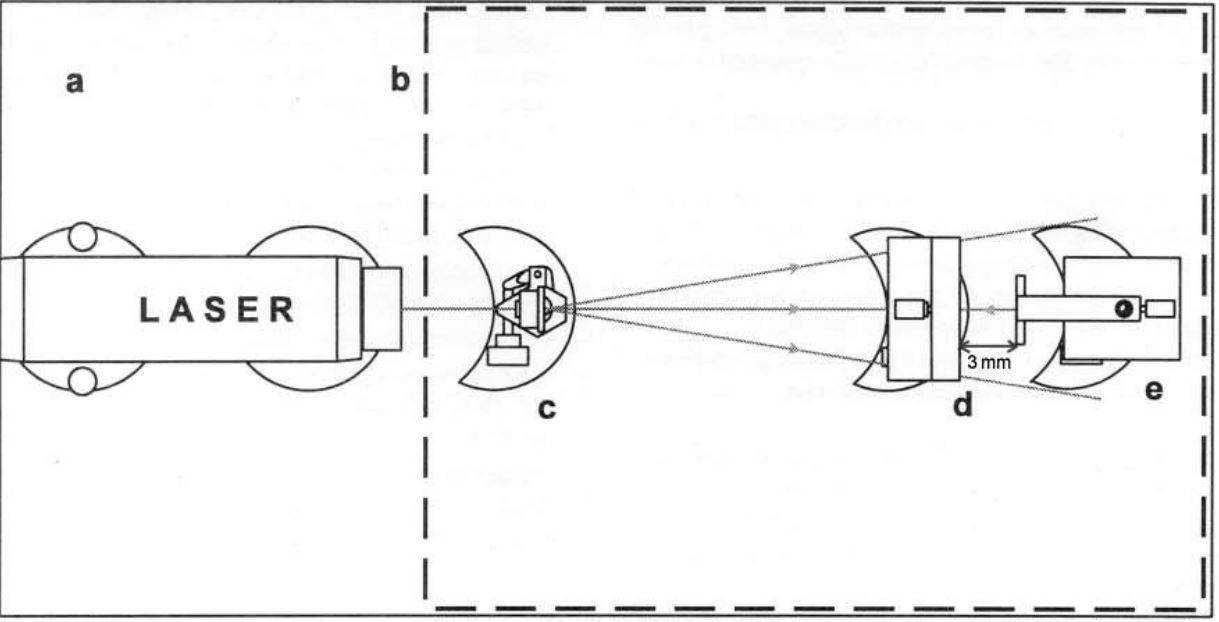
\includegraphics[scale=0.3]{Aufbau_holographie.jpg}
\label{Versuchsaufbau}
\end{figure}

\section{Geräteliste}
\begin{itemize}
\item HeNe Laser
\item Filmhalter
\item Objekthalter
\item Kugellinfe mit $f = \unit[2,7]{mm}$
\item Holographiefilm
\item diverse Materialen zum Entwickeln des Films
\end{itemize}


\section{Versuchsdurchführung}

Um das Hologramm zu erstellen, werden der Laser, die dicke Linse (c), der Objekthalter (e) und der Holographiefilm (d) wie oben dargestellt ausgerichtet. \\
Wenn der Laser angeschaltet wird, wird dieser zunächst von der Linse aufgeweitet, damit das ganze abzubildende Objekt bestrahlt wird. Das Licht wird nun vom Gegenstand auf dem Film zurückgeworfen und wir erhalten eine Abbildung des Objektes. \\
Wie früher die Aufnahme von Fotos, ist diese Art der Hologrammerstellung sehr empfindlich gegenüber äußeren Einflüssen. Diese sind z.B. eine Änderung der optischen Weglänge zwischen Objekt und Film durch Druck oder Temperaturänderung während der Aufnahme oder Erschütterungen des Aufbaus. 


\section{Ergebnisdiskussion}

Als abzubildendes Objekt haben wir einen Anhänger in Form eines Fahrrads genommen.

\begin{figure}[h]
	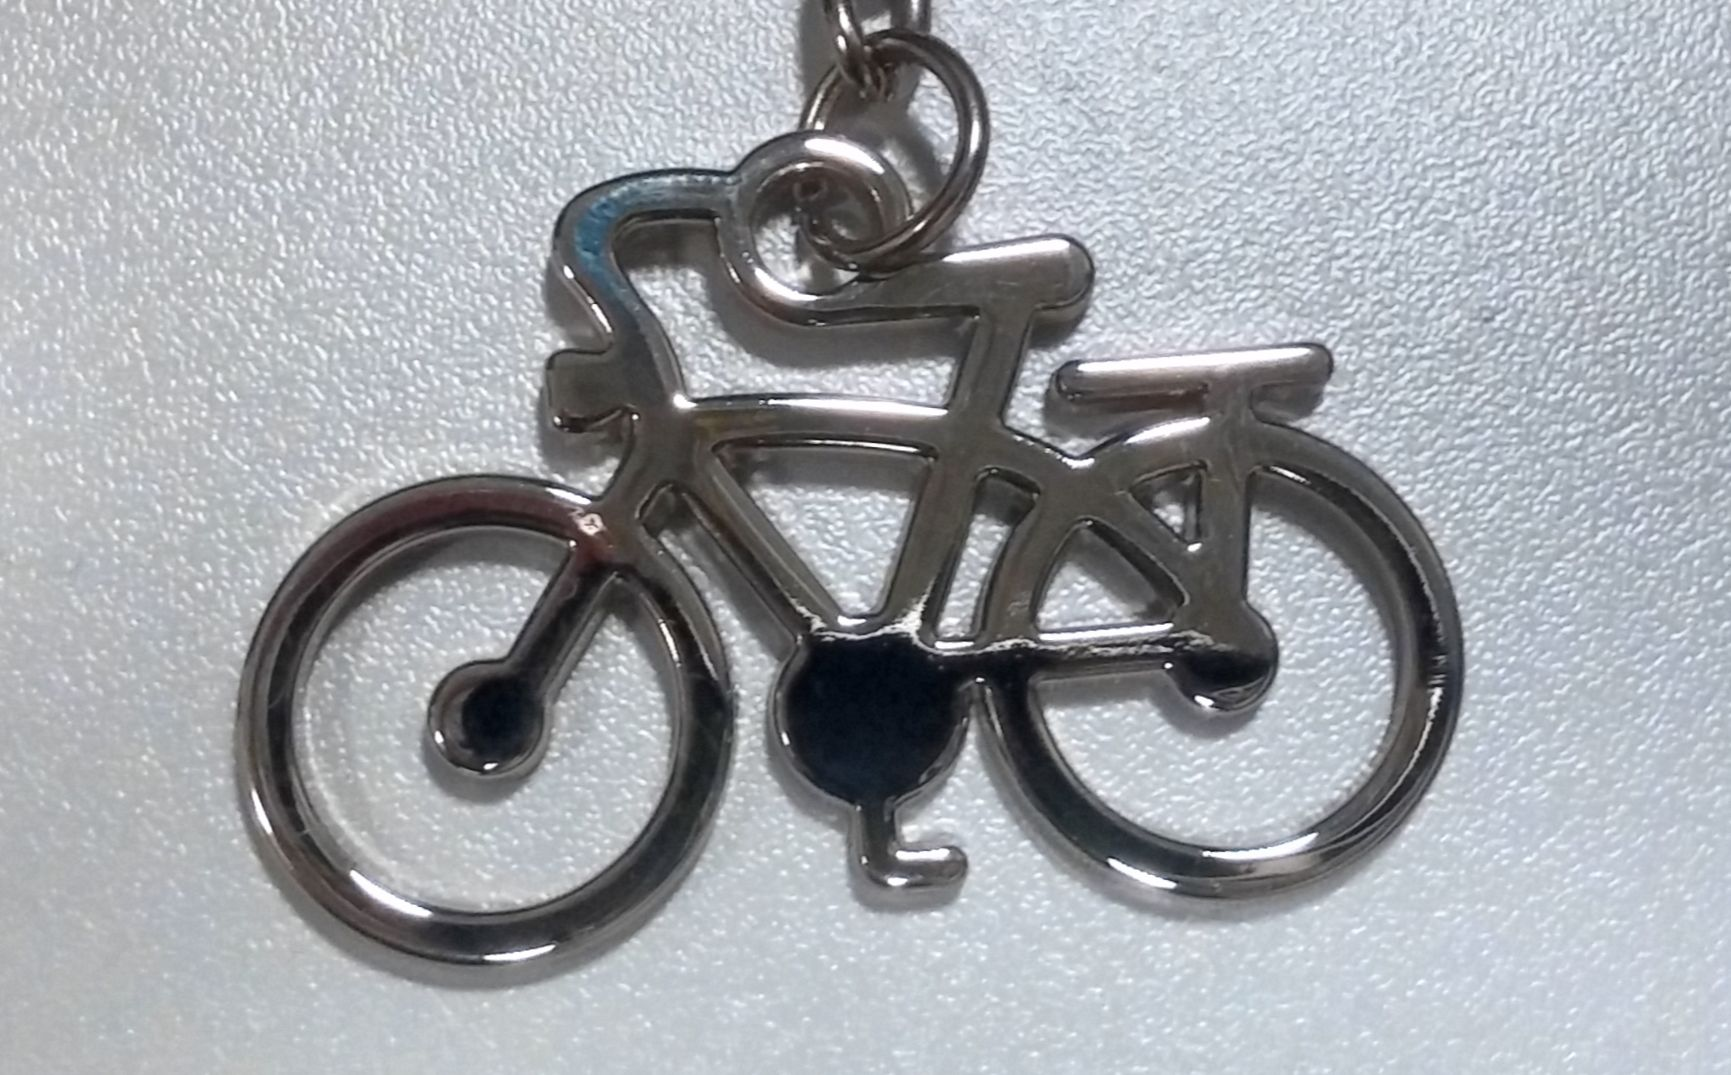
\includegraphics[scale=0.25]{Objekt.jpg}
	\label{Objekt}
	\caption{Unser verwendetes Objekt}
\end{figure}


Die Schwierigkeit bestand darin das Fahrrad als ganzes auf den Film zu bekommen, da es nur ganz knapp in das Fenster der Filmhalterung passte. Das Ergebnis ist unten eingeklebt. \\
Besonders gut kann man das Hinterrad und den Sattel erkennen, wenn man das Hologramm ein wenig verkippt, dann kann man auch den Rest recht gut erkennen.

\begin{figure}[h]
	\vspace{6cm}
	\label{Hologramm}
	\caption{hergestelltes Hologramm}
\end{figure}



\end{document}
